\section{Experimental Results}
\label{sec:results}

We evaluate all implemented models on the filtered CXR-LT-aligned test split. This section reports the experimental setup, main quantitative results, ablation studies, long-tail analysis, and qualitative Grad-CAM checks.

\subsection{Experimental Setup}
\label{subsec:results_setup}

Table~\ref{tab:experimental_setup} summarizes the experimental configuration and hyperparameter settings.

\begin{table}[H]
    \centering
    \caption{Experimental setup and hyperparameter configurations.}
    \label{tab:experimental_setup}
    \begin{tabular}{ll}
        \toprule
        \textbf{Parameter} & \textbf{Setting / Value} \\
        \midrule
        Image Resolution & $512 \times 512$ pixels \\
        Batch Size & 8 \\
        Effective Batch Size & 32 (batch size 8, gradient accumulation 4) \\
        Gradient Accumulation Steps & 4 \\
        Optimizer & AdamW (weight decay = $10^{-4}$) \\
        Base Learning Rate & $5\times10^{-5}$ (cosine annealing scheduler) \\
        Epochs & Maximum 50 epochs \\
        Early Stopping & Patience = 10 epochs (monitoring validation mAP) \\
        Loss Function & Asymmetric Loss (ASL) \\
        \bottomrule
    \end{tabular}
\end{table}

\paragraph{Model complexity under the frozen-text reference setting.}
Table~\ref{tab:model_complexity} compares the parameter counts of the original CaMCheX architecture and the proposed prior-aware model. The two systems use different image backbones and text encoders. CaMCheX uses ConvNeXt-Small and BioBERT, while the proposed model uses ConvNeXt-V2-Nano and BiomedVLP-CXR-BERT-specialized. Both text encoders are treated as frozen only for this parameter-count comparison. Therefore, the trainable count in this table excludes the text encoder. The comparison is used to show the approximate model size and training cost, not to claim an exact reproduction of CaMCheX.

\begin{table}[H]
    \centering
    \caption{Per-component parameter counts for the original CaMCheX architecture and the proposed prior-aware model. Text encoders are frozen; MLDecoder query embeddings (19{,}968) are also frozen.}
    \label{tab:model_complexity}
    \adjustbox{max width=\textwidth}{%
    \begin{tabular}{lrrr}
        \toprule
        \textbf{Component} & \textbf{CaMCheX} & \textbf{Proposed model} & \textbf{$\Delta$} \\
        \midrule
        \multicolumn{4}{l}{\textit{Image backbone}} \\
        \quad ConvNeXt-Small (frontal + lateral, 768ch) & 98.91M & -- & $-$98.91M \\
        \quad ConvNeXt-V2-Nano (frontal + lateral, 640ch) & -- & 29.96M & $+$29.96M \\
        \midrule
        \multicolumn{4}{l}{\textit{Text encoder (frozen, shared)}} \\
        \quad BioBERT (\texttt{dmis-lab/biobert-v1.1}) & 108.31M & -- & $-$108.31M \\
        \quad BiomedVLP-CXR-BERT-specialized & -- & 109.63M & $+$109.63M \\
        \midrule
        \multicolumn{4}{l}{\textit{Image projection}} \\
        \quad Conv2d 768$\to$768, k3 s2 & 5.31M & -- & $-$5.31M \\
        \quad MaxPool2d (stride 2) + Identity proj & -- & 0 & -- \\
        \midrule
        \multicolumn{4}{l}{\textit{Text projection}} \\
        \quad Linear 768$\to$1280 (2 tokens $\times$ 640) & -- & 0.98M & $+$0.98M \\
        \midrule
        \multicolumn{4}{l}{\textit{Vitals encoding}} \\
        \quad Text through shared BioBERT (vitals as text) & 0\textsuperscript{$\dagger$} & -- & -- \\
        \quad Dedicated 2-layer MLP (7$\to$256$\to$640) & -- & 0.17M & $+$0.17M \\
        \midrule
        \multicolumn{4}{l}{\textit{Prior context modules}} \\
        \quad Time-gap delta embedding (64 buckets) & -- & 6{,}144 & $+$6K \\
        \quad Prior label projection (26$\to$640) & -- & 20{,}736 & $+$21K \\
        \quad Per-modality LayerNorm ($\times$6) & -- & 9{,}216 & $+$9K \\
        \quad No-prior sentinel token & -- & 640 & $+$1K \\
        \quad Prior pooler (1-layer TransformerDecoder) & -- & 5.91M & $+$5.91M \\
        \midrule
        \multicolumn{4}{l}{\textit{Fusion}} \\
        \quad TransformerEncoder (2 layers, d=768) & 11.03M & -- & $-$11.03M \\
        \quad Fusion TransformerDecoder (2 layers, d=640) & -- & 11.82M & $+$11.82M \\
        \midrule
        \multicolumn{4}{l}{\textit{Classifier head}} \\
        \quad MLDecoder (query embed frozen) & 6.15M & 6.05M & $-$0.10M \\
        \midrule
        \midrule
        \textbf{Total} & \textbf{229.71M} & \textbf{164.58M} & \textbf{$-$65.13M} \\
        \textbf{Trainable} & \textbf{121.38M} & \textbf{54.93M} & \textbf{$-$66.45M} \\
        \bottomrule
    \end{tabular}%
    }
\end{table}

{\small \textsuperscript{$\dagger$} CaMCheX has no dedicated vitals module; vital signs are tokenized as a text string and encoded by the shared BioBERT encoder, incurring zero additional parameters beyond the text encoder itself.}

This parameter-count table compares architectural size under a frozen-text reference setting. The final reported model fine-tunes the CXR-BERT text encoder; therefore, its trainable parameter count is higher than the frozen-text count shown in Table~\ref{tab:model_complexity}.

\textbf{Image backbone.} The largest single reduction comes from replacing ConvNeXt-Small (49.45M per view, 768 channels) with ConvNeXt-V2-Nano (14.98M per view, 640 channels), saving 68.95M parameters across the dual-frontal/lateral encoders. This is the primary contributor to the overall parameter reduction and reflects the resource-constrained design choice.

\textbf{Text encoder.} The original CaMCheX uses BioBERT (108.31M), while the proposed model uses BiomedVLP-CXR-BERT-specialized (109.63M). Both are transformer-based clinical language models frozen during training; the 1.32M difference is negligible and does not affect the trainable parameter count. Critically, CaMCheX uses this single shared encoder for both the clinical indication text and the vital signs (encoded as a text string), whereas the proposed model routes vitals through a separate dedicated projector.

\textbf{Vitals encoding.} In CaMCheX, the 7 vital signs (temperature, heart rate, respiratory rate, O2 saturation, systolic/diastolic BP, gender) are formatted as a natural-language string and passed through BioBERT alongside the clinical indication, incurring no additional parameters. The proposed model instead uses a compact 2-layer MLP (0.17M) that maps the 7 scalar values directly to a single 640-dimensional token, avoiding the overhead of tokenizing and encoding vitals through a 108M-parameter transformer.

\textbf{Image projection.} CaMCheX projects 768-channel backbone features through a strided Conv2d (5.31M) to match the transformer width. The proposed model operates natively at 640 dimensions ($d_\text{model} = 640$), replacing the convolution with a parameter-free 2$\times$2 max-pool.

\textbf{Prior context modules.} These are unique to the proposed model: a 64-bucket time-gap embedding (6K), a prior label projection from 26 classes to 640 dimensions (21K), six per-modality LayerNorms (9K), a no-prior sentinel token (640), and a 1-layer prior pooler TransformerDecoder (5.91M) with 16 learned query latents that compress the prior memory via cross-attention.

\textbf{Fusion mechanism.} CaMCheX uses a 2-layer TransformerEncoder (11.03M) that self-attends over all concatenated tokens. The proposed model replaces this with a 2-layer Fusion TransformerDecoder (11.82M) where current tokens query prior-pooled latents via asymmetric cross-attention.

Overall, the proposed model reduces the total parameter count from 229.71M to 164.58M ($-$65.13M, about $-$28\%). Under the frozen-text comparison, the trainable parameter count is reduced from 121.38M to 54.93M ($-$66.45M, about $-$55\%). This reduction mainly comes from the smaller image backbone. Even after adding prior pooling, cross-attention fusion, and a dedicated vitals projector, the proposed model remains smaller and cheaper to train than the CaMCheX-style reference architecture.


\subsection{Main Performance of the Proposed Model}
\label{subsec:results_quantitative}

We evaluate all models using mAP and mAUROC. Because the label distribution is long-tailed, we also report mAP by frequency group: head, medium, and tail. These groups follow the label-frequency split described in the data analysis section. Table~\ref{tab:ours_main_results} compares the three model configurations trained and tested in this work.

\begin{table}[H]
    \centering
    \caption{Main test-set performance of the implemented models in this work.}
    \label{tab:ours_main_results}
    \begin{tabular}{lccccc}
        \toprule
        Model & mAP & mAUROC & Head mAP & Medium mAP & Tail mAP \\
        \midrule
        Image-only baseline & 0.3246 & 0.8123 & 0.5841 & 0.2285 & 0.0827 \\
        Multimodal without prior & 0.4098 & 0.8732 & 0.7116 & 0.3693 & 0.1586 \\
        Proposed prior-aware multimodal model & 0.5662 & 0.9026 & 0.7739 & 0.5268 & 0.4076 \\
        \bottomrule
    \end{tabular}
\end{table}

\begin{table}[H]
    \centering
    \caption{Per-group mAUROC breakdown for the main models. Head and medium mAUROC were not logged for the image-only run.}
    \label{tab:ours_main_results_auroc}
    \begin{tabular}{lcccc}
        \hline
        Model & mAUROC & Head mAUROC & Medium mAUROC & Tail mAUROC \\
        \hline
        Image-only baseline & 0.8123 & -- & -- & 0.7998 \\
        Multimodal without prior & 0.8732 & 0.8718 & 0.8642 & 0.8860 \\
        Proposed prior-aware multimodal model & 0.9026 & 0.8944 & 0.8937 & 0.9218 \\
        \hline
    \end{tabular}
\end{table}

The results show three main patterns.

\textbf{Multimodal context improves performance.} Adding clinical text and vital signs to the image-only baseline raises mAP from 0.3246 to 0.4098 and mAUROC from 0.8123 to 0.8732. This shows that the model benefits from clinical context in addition to the radiograph.

\textbf{Prior-aware fusion gives the largest gain.} Adding prior-study context increases mAP from 0.4098 to 0.5662 and mAUROC from 0.8732 to 0.9026. This is a gain of 0.1564 mAP over the no-prior multimodal baseline.

\textbf{Tail classes improve the most.} Tail mAP increases from 0.0827 in the image-only baseline to 0.4076 in the proposed model. Compared with the no-prior multimodal baseline, tail mAP increases from 0.1586 to 0.4076. This suggests that clinical context and prior-study information are especially useful for rare labels, although this should be interpreted together with the ablation results.

\subsection{Comparison with Reference Methods}
\label{subsec:results_reference_comparison}

We compare our results with CheXFusion \cite{kim2023chexfusion} and CaMCheX \cite{sloan2025camchex} only as external context. This is not a controlled comparison. The published methods use different dataset scale, preprocessing, resolution, training strategy, and pretraining. Our results are also measured on the filtered CXR-LT-aligned thesis cohort rather than a full benchmark reproduction.

\begin{table}[H]
    \centering
    \caption[Contextual comparison with published reference results]{Contextual comparison with published reference results. These published results are not directly comparable because they use larger datasets, higher resolutions, different preprocessing, and additional pretraining.}
    \label{tab:contextual_comparison}
    \adjustbox{max width=\textwidth}{%
    \begin{tabular}{lccc}
        \hline
        Method & Setting (Resolution) & mAP & mAUROC \\
        \hline
        \begin{tabular}[t]{@{}l@{}}CheXFusion \cite{kim2023chexfusion} (ConvNeXt-S, multi-view Transformer fusion, \\ ML-Decoder, weighted ASL, 1024 $\times$ 1024 input resolution)\end{tabular} & Published CXR-LT 2023 & 0.372 & 0.850 \\
        CaMCheX \cite{sloan2025camchex} & Published CXR-LT 2023 ($1024 \times 1024$) & 0.576 & 0.916 \\
        Proposed model & Our setting ($512 \times 512$) & 0.5662 & 0.9026 \\
        \hline
    \end{tabular}%
    }
\end{table}

Table~\ref{tab:contextual_comparison} places the proposed model beside published CXR-LT reference results. The proposed model reaches 0.5662 mAP and 0.9026 mAUROC in our filtered setting. These values are close to the published CaMCheX CXR-LT 2023 result of 0.576 mAP and 0.916 mAUROC. However, the numbers should not be read as a leaderboard comparison because the experimental settings are different. The main controlled evidence in this thesis comes from the models trained and evaluated under the same filtered cohort in Table~\ref{tab:ours_main_results} and Table~\ref{tab:ablation_unified}.

\subsection{Ablation Study}
\label{subsec:results_ablation}

Table~\ref{tab:ablation_unified} summarizes the ablation and development runs performed in this work. The table has three groups. \emph{Modality ablation} removes one input modality at a time. \emph{Incremental model variants} report the available runs as prior-aware components and the final training setting were added. \emph{Channel encoding ablation} compares the engineered three-channel image input with a simple \texttt{gray3} baseline. Published CaMCheX numbers are not included because they are external references, not controlled ablations. Due to limited compute, not every later training choice is isolated under an otherwise identical run; therefore, the incremental-variant rows should be interpreted as development evidence rather than a complete causal decomposition.

\begin{table}[H]
\centering
\caption[Unified ablation study]{Unified ablation study on the filtered CXR-LT-aligned test split. All rows are runs from this work. Intermediate component rows lack per-group mAP because those configurations were evaluated with aggregate metrics only.}
\label{tab:ablation_unified}
\adjustbox{max width=\textwidth}{%
\begin{tabular}{llccccc}
\toprule
\textbf{Study} & \textbf{Configuration} & \textbf{mAP} & \textbf{mAUROC} & \textbf{Head mAP} & \textbf{Medium mAP} & \textbf{Tail mAP} \\
\midrule
\multicolumn{7}{l}{\textit{A.\ Modality Ablation} (prior-aware architecture fixed, input modalities varied)} \\
\midrule
& Full (image + clinical text + vitals + prior) & 0.5662 & 0.9026 & 0.7739 & 0.5268 & 0.4076 \\
& Clinical text dropped (image + vitals + prior) & 0.3404 & 0.8121 & 0.6083 & 0.2524 & 0.1827 \\
& Vitals dropped (image + clinical text + prior) & 0.5666 & 0.9023 & 0.7738 & 0.5267 & 0.4091 \\
& Image-only baseline & 0.3246 & 0.8123 & 0.5841 & 0.2285 & 0.0827 \\
\midrule
\multicolumn{7}{l}{\textit{B.\ Incremental Model Variants} (components added across available runs)} \\
\midrule
& Image-only baseline & 0.3246 & 0.8123 & 0.5841 & 0.2285 & 0.0827 \\
& + Multimodal inputs (no prior) & 0.4098 & 0.8732 & 0.7116 & 0.3693 & 0.1586 \\
& + Prior study (no time-gap embedding) & 0.4479 & 0.8845 & -- & -- & -- \\
& + Time-gap embedding (no prior dropout) & 0.4668 & 0.8901 & -- & -- & -- \\
& + Prior dropout & 0.4950 & 0.8985 & 0.7428 & 0.4760 & 0.2708 \\
& Final model with trainable text encoder & 0.5662 & 0.9026 & 0.7739 & 0.5268 & 0.4076 \\
\midrule
\multicolumn{7}{l}{\textit{C.\ Channel Encoding Ablation} (architecture and training fixed)} \\
\midrule
& Engineered multi-channel (full inputs) & 0.5662 & 0.9026 & 0.7739 & 0.5268 & 0.4076 \\
& Plain \texttt{gray3} (full inputs) & 0.5633 & 0.9000 & 0.7705 & 0.5235 & 0.4059 \\
& Engineered multi-channel (clinical text dropped) & 0.3404 & 0.8121 & 0.6083 & 0.2524 & 0.1827 \\
& Plain \texttt{gray3} (clinical text dropped) & 0.3367 & 0.8094 & 0.6054 & 0.2477 & 0.1791 \\
\bottomrule
\end{tabular}%
}
\end{table}

\subsubsection{Modality Ablation}
\label{subsubsec:ablation_modality}

Removing clinical text causes the largest drop, from 0.5662 to 0.3404 mAP. This shows that clinical indication text carries strong predictive information. This information is clinically available before interpretation, but it may also contain strong diagnostic cues such as suspected disease names. Therefore, the gain should be interpreted as the value of clinical context, with a possible cueing effect from the indication text. Dropping vital signs has almost no effect: mAP changes from 0.5662 to 0.5666. This small difference is within expected run-to-run noise and should not be interpreted as evidence that vital signs improve or hurt performance.

\subsubsection{Incremental Model Variants}
\label{subsubsec:ablation_components}

Group B reports incremental model variants trained during development. These rows show how performance changed as prior-aware components and the final training setting were added. They should not be read as a complete causal decomposition because not every final training choice was isolated in a separate controlled run.

\textbf{Multimodal inputs.} Adding clinical text and vital signs to the image-only baseline improves mAP from 0.3246 to 0.4098 and mAUROC from 0.8123 to 0.8732. This is the first major gain.

\textbf{Prior study tokens.} Adding prior-study information without time-gap embeddings improves mAP from 0.4098 to 0.4479 and mAUROC from 0.8732 to 0.8845. This shows that historical context is useful even before explicit time modelling is added.

\textbf{Time-gap embeddings.} Adding time-gap embeddings improves mAP from 0.4479 to 0.4668 and mAUROC from 0.8845 to 0.8901. This suggests that the model benefits from knowing whether a prior study is recent or old.

\textbf{Prior dropout.} Adding prior dropout improves mAP from 0.4668 to 0.4950 and mAUROC from 0.8901 to 0.8985. This supports the use of prior dropout to reduce over-reliance on historical information.

\textbf{Final training setting.} The final model improves mAP from 0.4950 to 0.5662 and mAUROC from 0.8985 to 0.9026. This final setting keeps the full prior-aware multimodal architecture and fine-tunes the radiology-domain text encoder instead of using frozen text features. Because this final row also reflects the selected training setting, it should be interpreted as the performance of the final selected model rather than as a causal measurement of one isolated component.

\subsubsection{Input Channel Encoding Ablation}
\label{subsubsec:ablation_channels}

The image encoder expects a three-channel input, which leaves open the question of how a single-channel chest radiograph should be expanded to fill those channels. The proposed model uses an engineered multi-channel encoding, where each channel carries a distinct, separately-normalized representation. The plain \texttt{gray3} baseline simply replicates the raw grayscale image (normalized with mean $0.4721$ and standard deviation $0.3037$) across all three channels.

The engineered encoding and gray3 baseline perform almost the same: the engineered encoding is marginally higher on macro mAP ($0.5662$ vs.\ $0.5633$), macro mAUROC ($0.9026$ vs.\ $0.9000$), and tail mAP ($0.4076$ vs.\ $0.4059$). The clinical-text-dropped floor is likewise within noise ($0.3404$ vs.\ $0.3367$ macro mAP). The difference is small, so channel encoding is not a major driver of the final result. The engineered encoding is kept as the selected configuration in this thesis, but the ablation shows that a simple \texttt{gray3} input is a strong and simpler alternative. Most of the performance gain comes from multimodal context and prior-aware components, not from hand-crafted channel encoding.

\subsection{Long-Tail Analysis}
\label{subsec:results_longtail}

Tail classes show the clearest improvement. Tail mAP increases from 0.0827 for the image-only baseline to 0.4076 for the proposed model. Compared with the no-prior multimodal baseline, tail mAP increases from 0.1586 to 0.4076. Tail mAUROC also increases from 0.7998 to 0.9218.

Two factors may explain this pattern. First, some rare labels have strong cues in the clinical indication text. For example, an indication may mention evaluation for hiatal hernia or free air. These cues can help the model rank rare labels even when there are few visual examples. Second, prior studies can help with stable or chronic findings, because the model can compare the current study with historical information. These explanations are plausible, but they should be treated as interpretation rather than causal proof.

\subsection{Grad-CAM Qualitative Analysis}
\label{subsec:results_qualitative}

We use three case studies as qualitative sanity checks: Support Devices (head), Nodule (medium), and Hernia (tail). These Grad-CAM and text-attribution examples are not clinical explanations. They are used only to inspect whether the model uses plausible image regions and text cues.

\subsubsection{Case Study 1 (Head): Support Devices}
\label{subsubsec:case_support_devices}

For Support Devices, Figure~\ref{fig:fig_support_devices_gradcam} shows the Grad-CAM visual attribution maps, Figure~\ref{fig:support_devices_text} shows the word-level text attributions, and Figure~\ref{fig:support_devices_modality} shows the modality attribution share. The Grad-CAM map concentrates on regions containing visible tubes and lines, which is consistent with the target label. The text attribution highlights device-related indication terms, suggesting that the model uses both visual and clinical context. However, strong reliance on indication text may also increase shortcut risk if device presence is frequently mentioned before imaging.

\begin{figure}[H]
     \centering
     \begin{subfigure}[b]{0.85\textwidth}
          \centering
          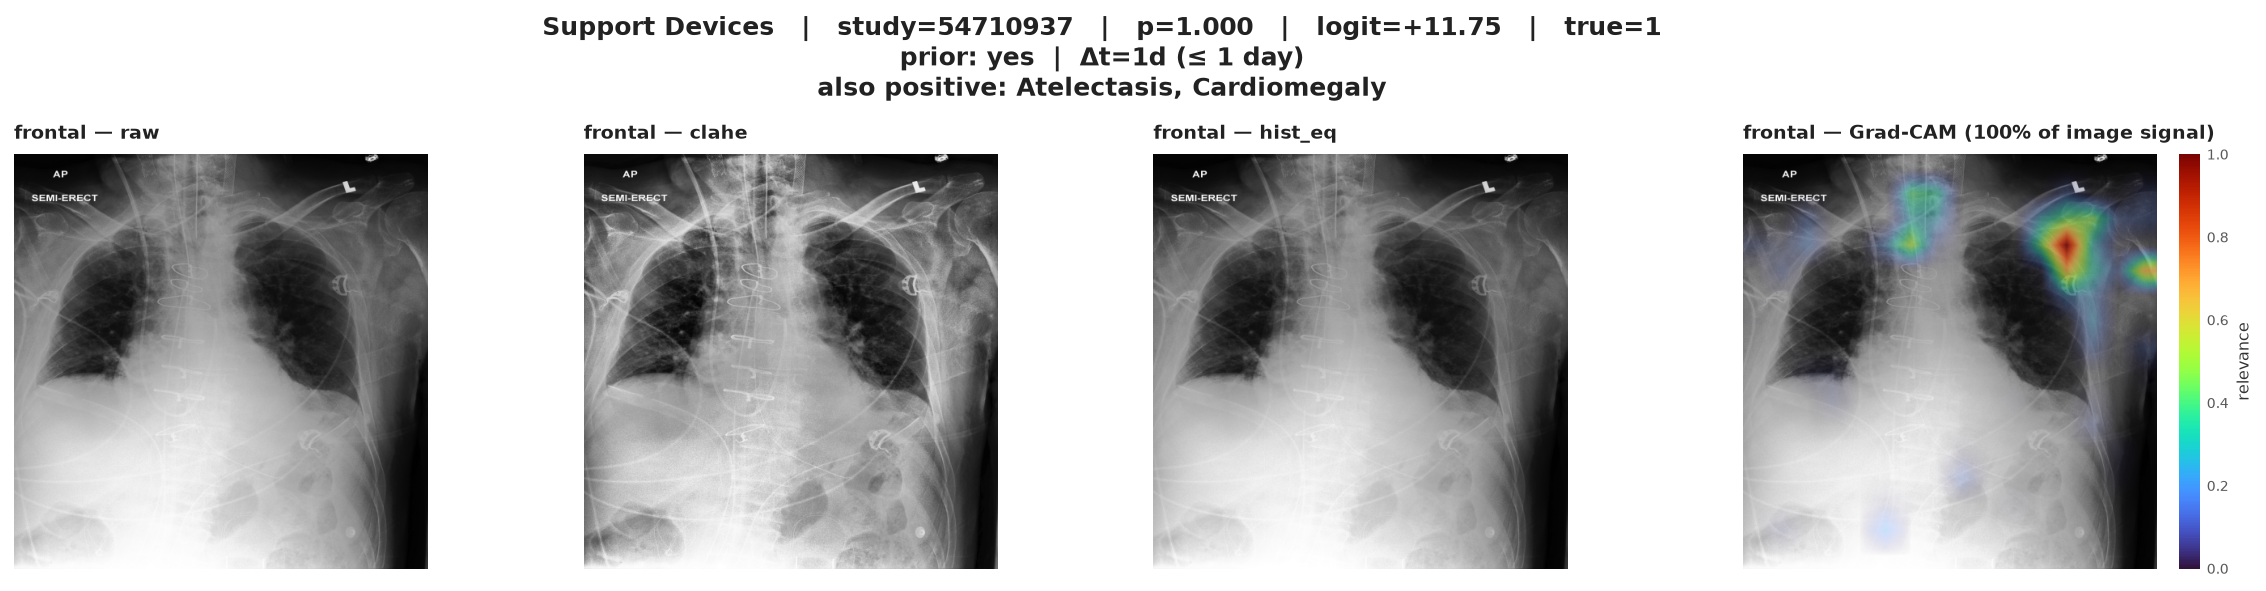
\includegraphics[width=\textwidth]{img/support_devices_gradcam.png}
          \caption{Current Target Image Attribution}
          \label{fig:support_devices_cur}
     \end{subfigure}
     \vspace{0.3cm}

     \begin{subfigure}[b]{0.85\textwidth}
          \centering
          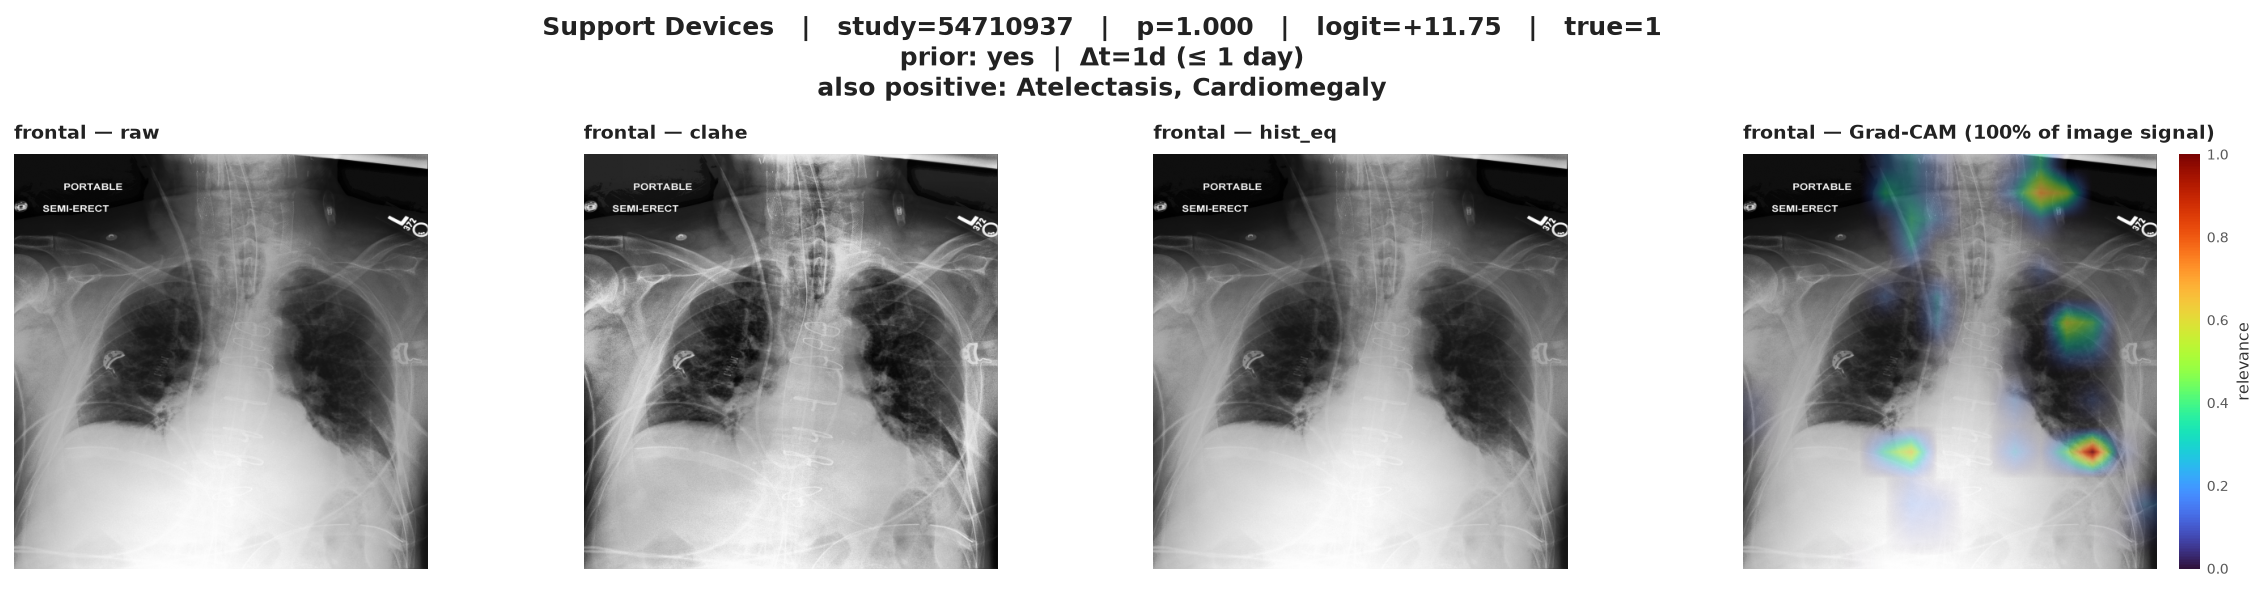
\includegraphics[width=\textwidth]{img/support_devices_prior.png}
          \caption{Prior Image Attribution}
          \label{fig:support_devices_prv}
     \end{subfigure}
        \caption[Grad-CAM Visual Attribution Maps for Support Devices]{Grad-CAM Visual Attribution Maps for Support Devices. (a) Current target image attribution. (b) Prior image attribution.}
        \label{fig:fig_support_devices_gradcam}
\end{figure}

\begin{figure}[H]
    \centering
    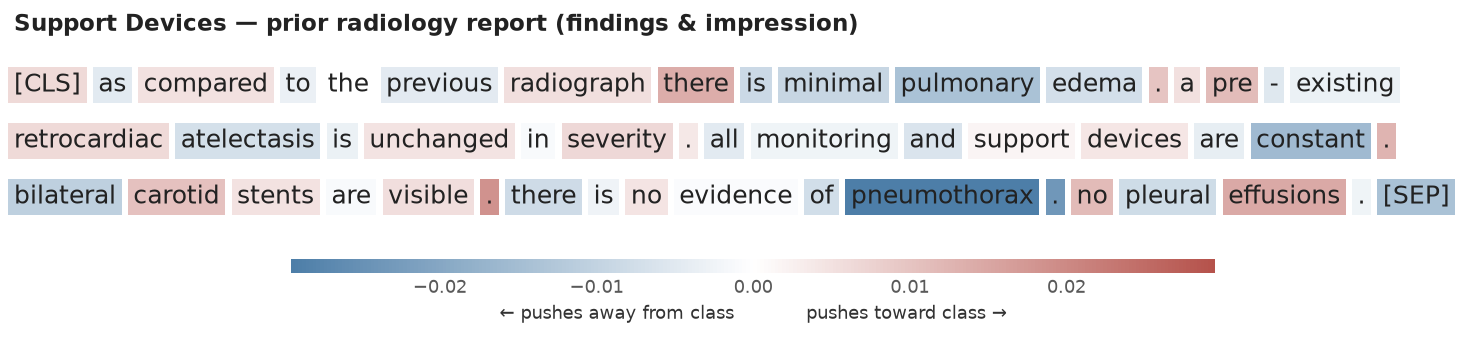
\includegraphics[width=0.85\textwidth]{img/support_devices_text.png}
    \caption[Word-Level Clinical Text Attributions for Support Devices]{Word-Level Clinical Text Attributions for Support Devices.}
    \label{fig:support_devices_text}
\end{figure}

\begin{figure}[H]
    \centering
    \begin{subfigure}[b]{0.48\textwidth}
        \centering
        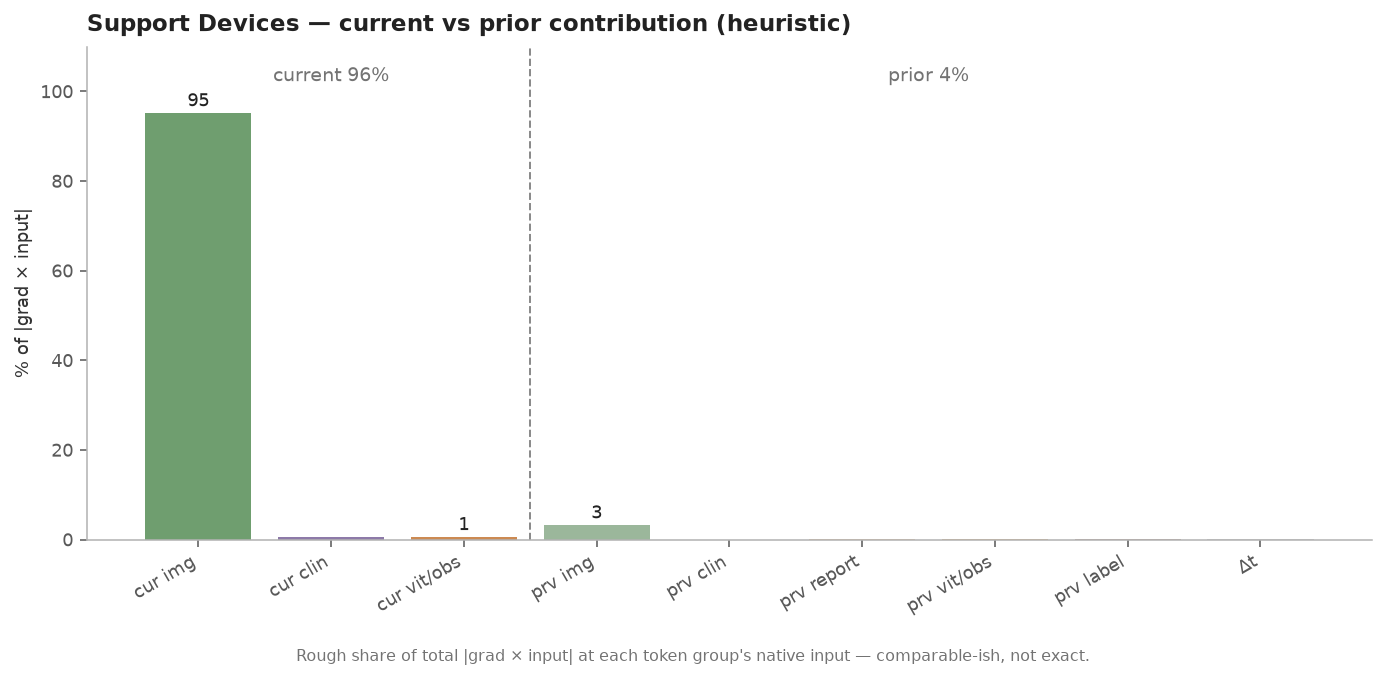
\includegraphics[width=\textwidth]{img/support_devices_modality.png}
        \caption{Normal Scale}
        \label{fig:support_devices_modality_normal}
    \end{subfigure}
    \hfill
    \begin{subfigure}[b]{0.48\textwidth}
        \centering
        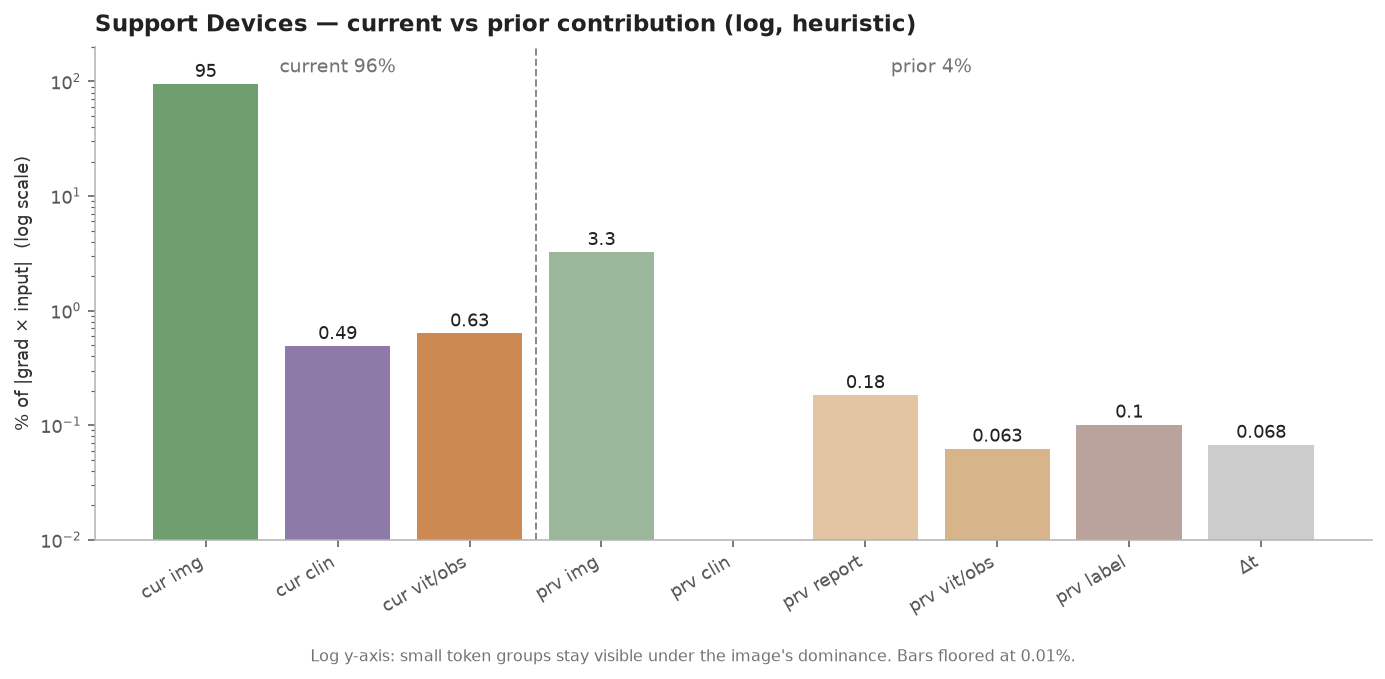
\includegraphics[width=\textwidth]{img/support_devices_modality_log.png}
        \caption{Log Scale}
        \label{fig:support_devices_modality_log}
    \end{subfigure}
    \caption[Modality Attribution Share for Support Devices]{Modality Attribution Share for Support Devices. (a) Normal scale. (b) Log scale.}
    \label{fig:support_devices_modality}
\end{figure}

\subsubsection{Case Study 2 (Medium): Nodule}
\label{subsubsec:case_nodule}

For Nodule, Figure~\ref{fig:fig_nodule_gradcam} shows the Grad-CAM visual attribution maps, Figure~\ref{fig:nodule_text} shows the word-level text attributions, and Figure~\ref{fig:nodule_modality} shows the modality attribution share. The Grad-CAM map focuses on lung parenchyma regions where nodules are typically found, which is clinically plausible. The text attribution highlights terms related to nodule evaluation, suggesting the model integrates visual findings with clinical indication context. However, nodule detection remains sensitive to resolution, and subtle findings may be missed at the $512 \times 512$ input resolution used in this work.

\begin{figure}[H]
     \centering
     \begin{subfigure}[b]{0.85\textwidth}
          \centering
          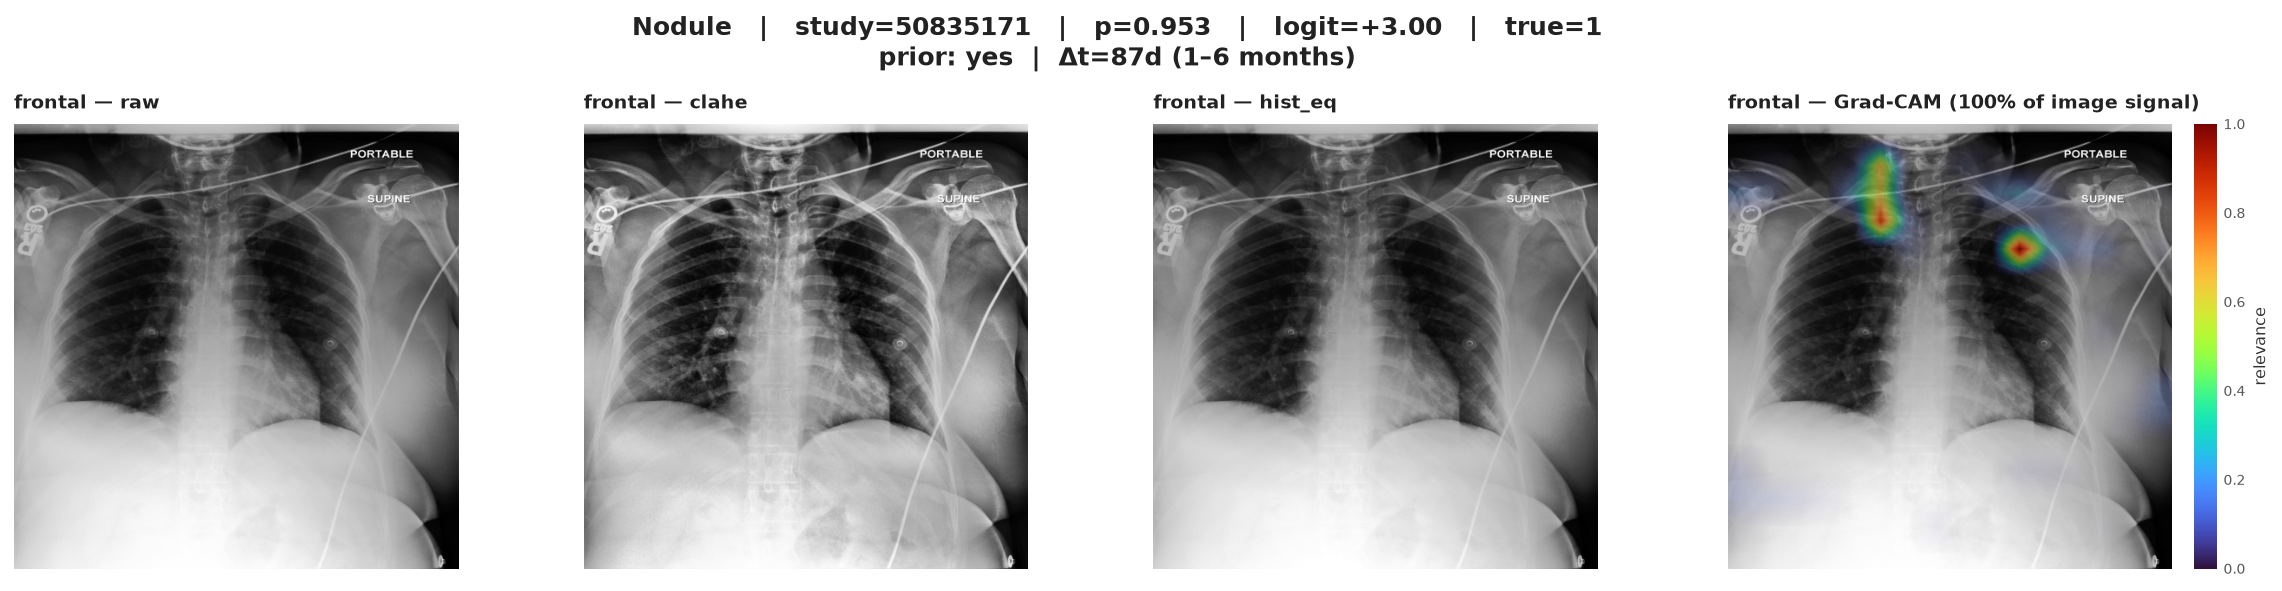
\includegraphics[width=\textwidth]{img/nodule_gradcam.png}
          \caption{Current Target Image Attribution}
          \label{fig:nodule_cur}
     \end{subfigure}
     \vspace{0.3cm}
     
     \begin{subfigure}[b]{0.85\textwidth}
          \centering
          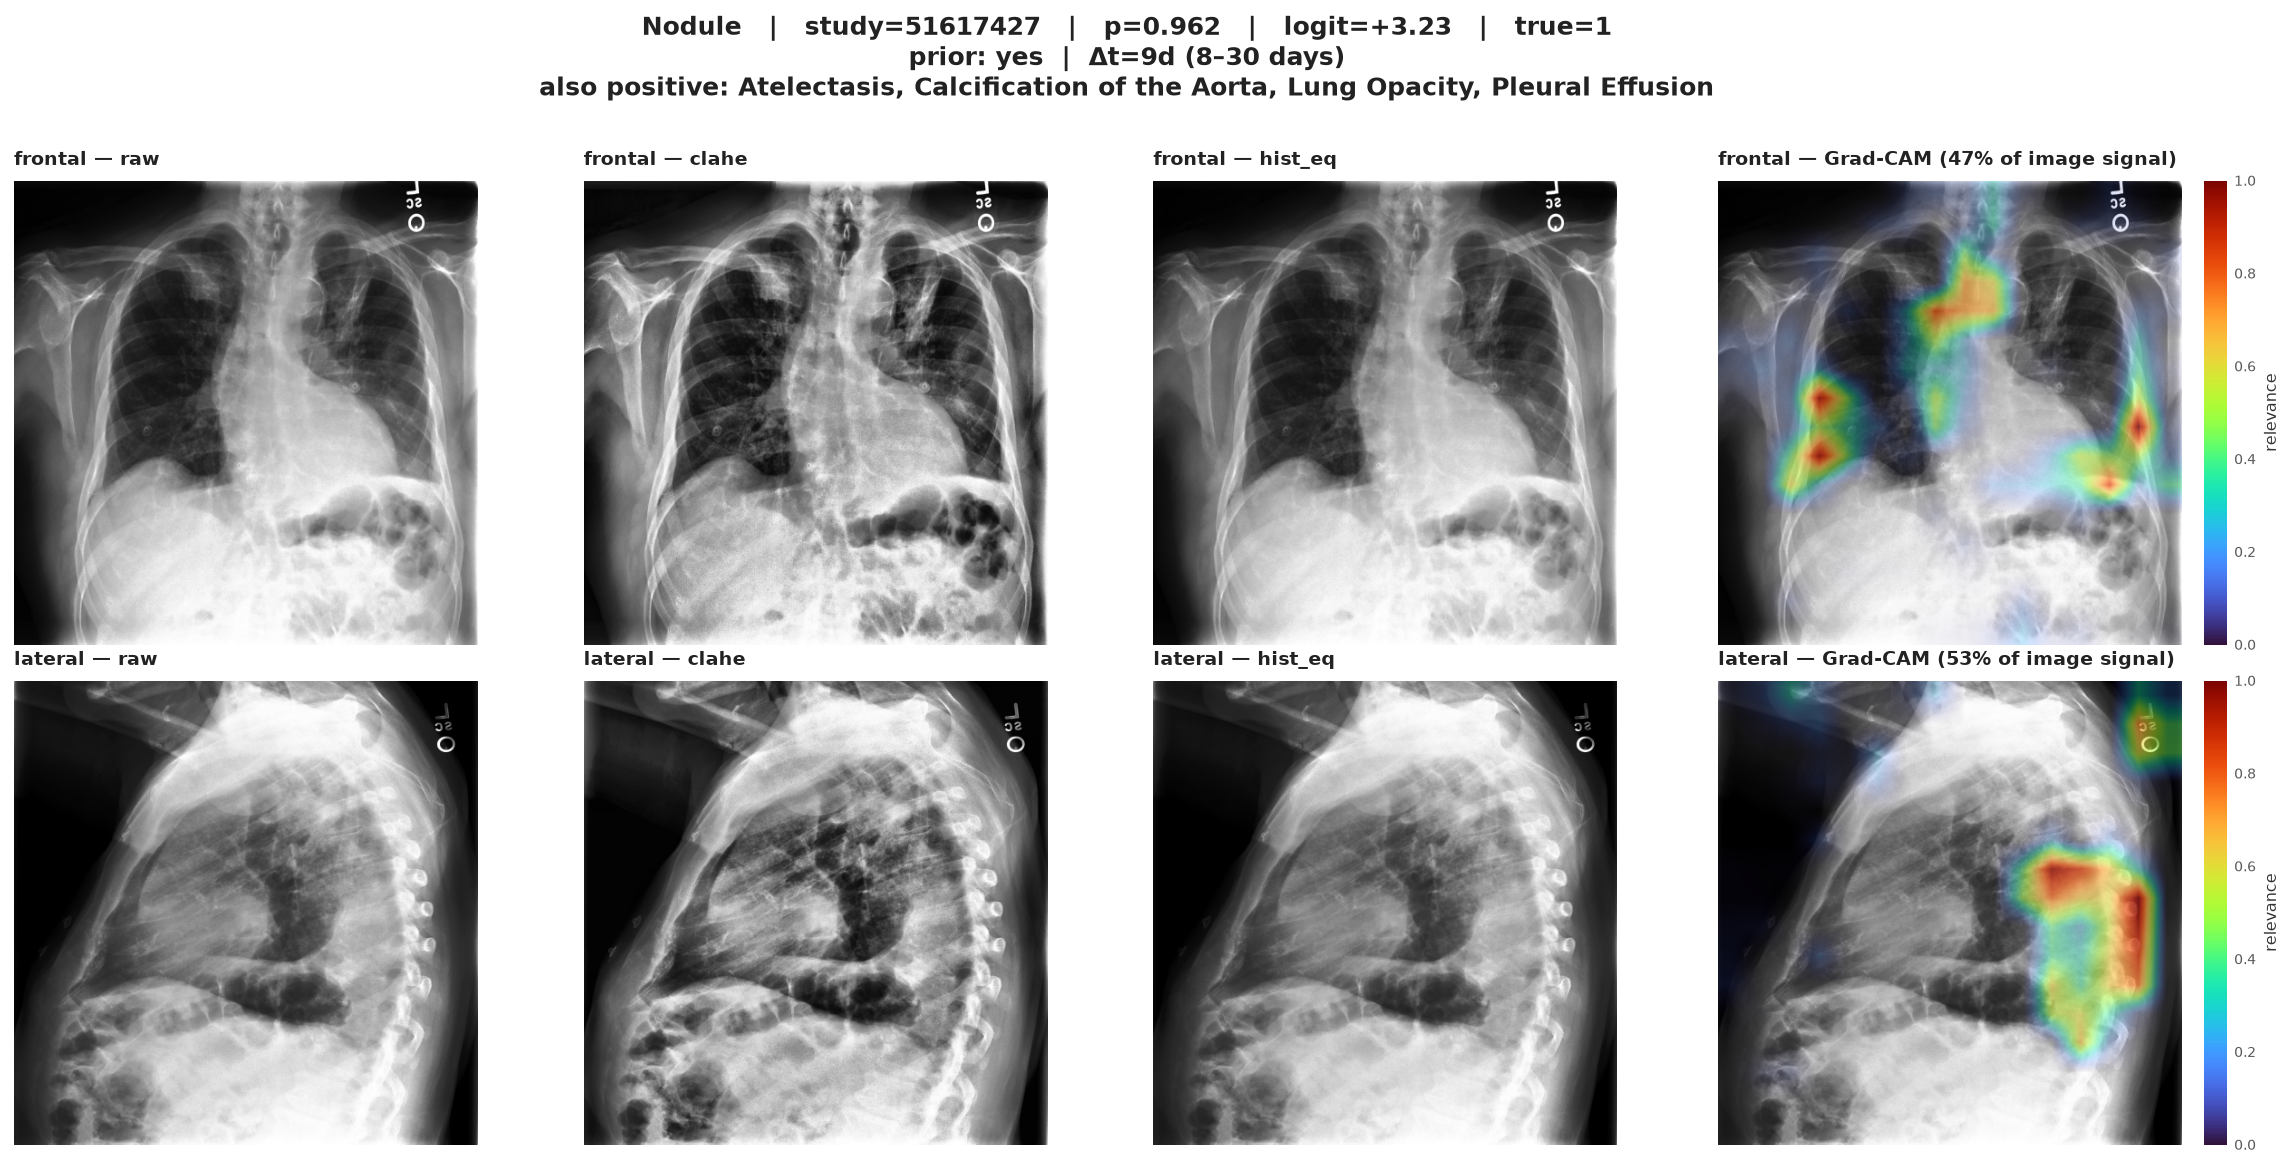
\includegraphics[width=\textwidth]{img/nodule_prior.png}
          \caption{Prior Image Attribution}
          \label{fig:nodule_prv}
     \end{subfigure}
        \caption[Grad-CAM Visual Attribution Maps for Nodule]{Grad-CAM Visual Attribution Maps for Nodule. (a) Current target image attribution. (b) Prior image attribution.}
        \label{fig:fig_nodule_gradcam}
\end{figure}

\begin{figure}[H]
    \centering
    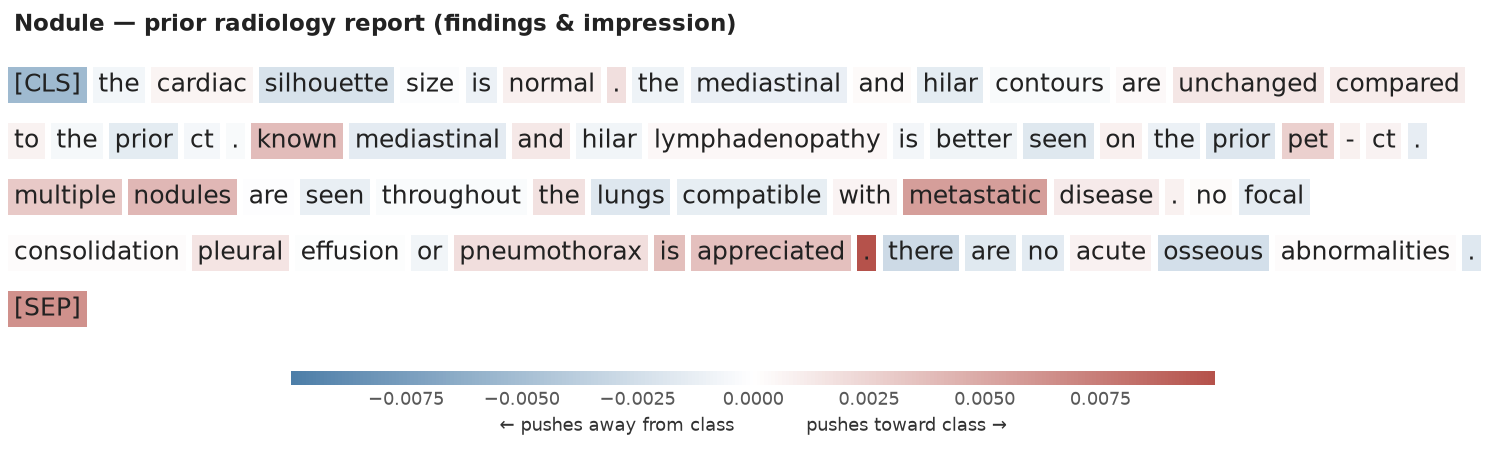
\includegraphics[width=0.85\textwidth]{img/nodule_text.png}
    \caption[Word-Level Clinical Text Attributions for Nodule]{Word-Level Clinical Text Attributions for Nodule.}
    \label{fig:nodule_text}
\end{figure}

\begin{figure}[H]
    \centering
    \begin{subfigure}[b]{0.48\textwidth}
        \centering
        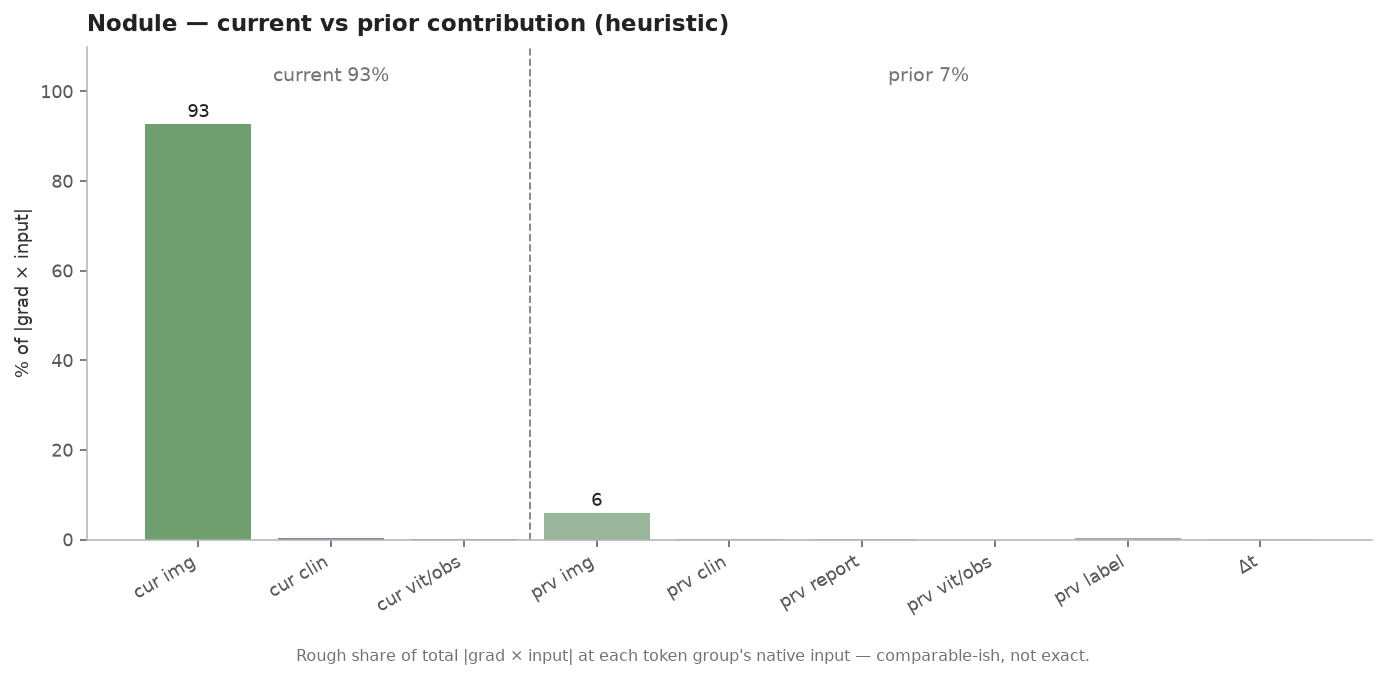
\includegraphics[width=\textwidth]{img/nodule_modality.png}
        \caption{Normal Scale}
        \label{fig:nodule_modality_normal}
    \end{subfigure}
    \hfill
    \begin{subfigure}[b]{0.48\textwidth}
        \centering
        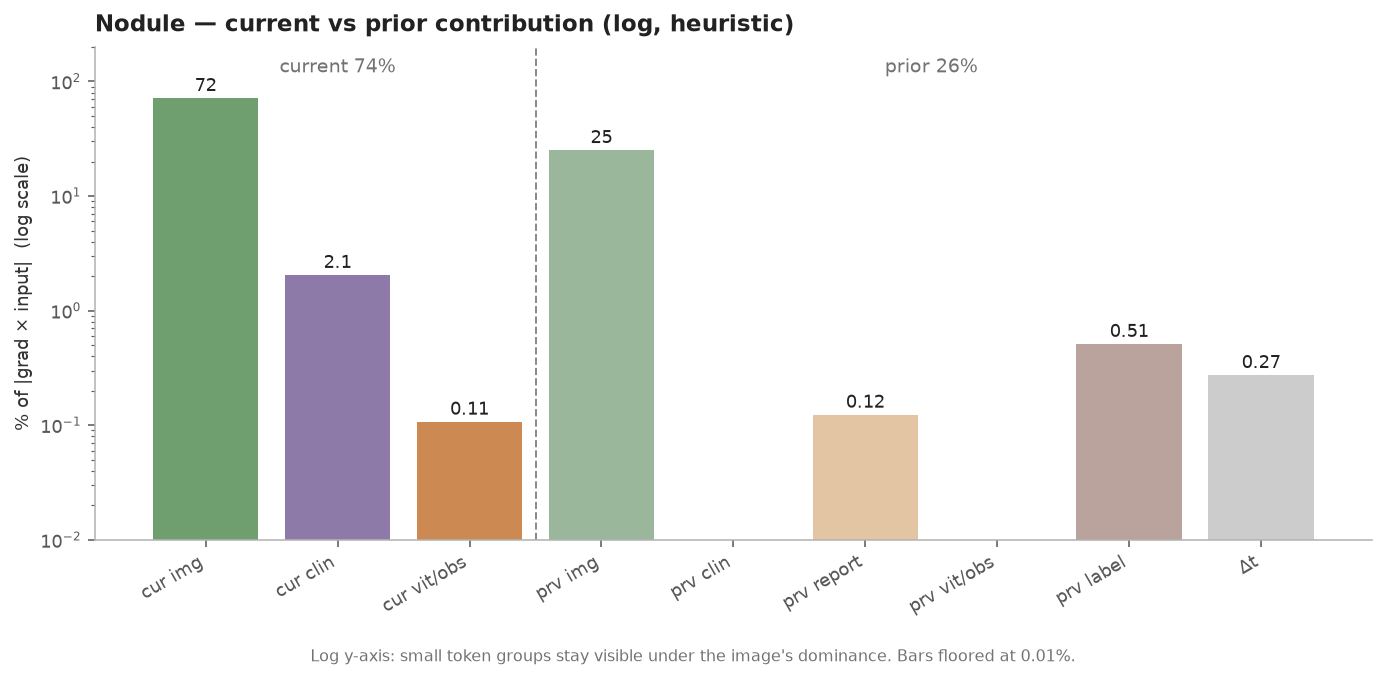
\includegraphics[width=\textwidth]{img/nodule_modality_log.png}
        \caption{Log Scale}
        \label{fig:nodule_modality_log}
    \end{subfigure}
    \caption[Modality Attribution Share for Nodule]{Modality Attribution Share for Nodule. (a) Normal scale. (b) Log scale.}
    \label{fig:nodule_modality}
\end{figure}

\subsubsection{Case Study 3 (Tail): Hernia}
\label{subsubsec:case_hernia}

For Hernia, Figure~\ref{fig:fig_hernia_gradcam} shows the current-image Grad-CAM map, Figure~\ref{fig:hernia_text} shows the word-level text attribution, and Figure~\ref{fig:hernia_modality} shows the modality attribution share. This case has no linked prior study, so it tests the model's no-prior fallback rather than direct comparison with a prior image. The Grad-CAM map attends to the lower thoracic and upper abdominal region, which is plausible for hiatal hernia. The text attribution highlights hernia-related indication terms, suggesting that clinical text provides useful evidence for this rare label.

\begin{figure}[H]
     \centering
     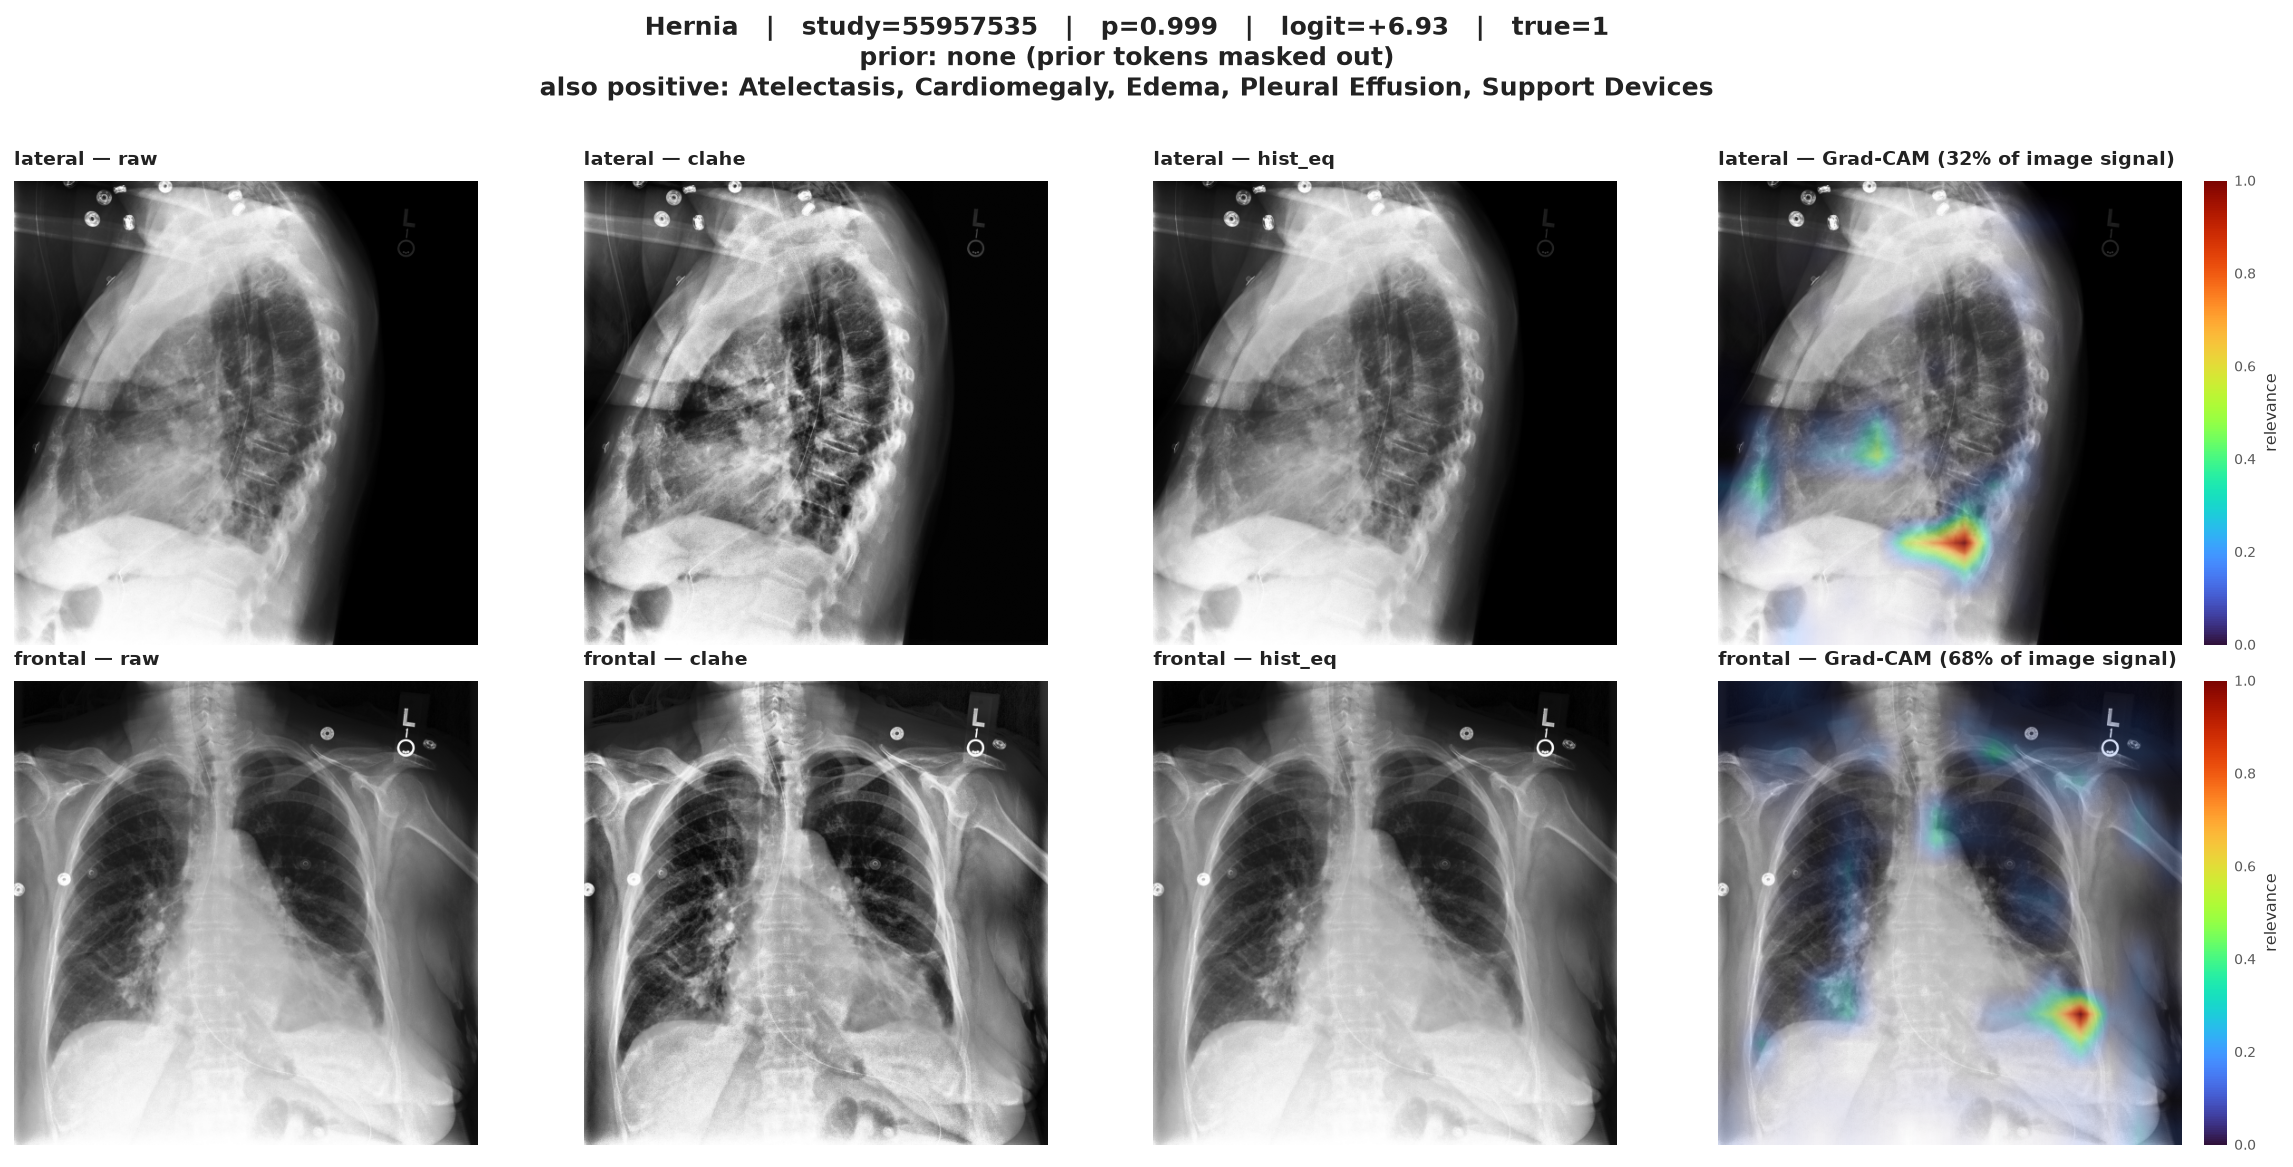
\includegraphics[width=0.85\textwidth]{img/hernia_gradcam.png}
     \caption[Grad-CAM Visual Attribution for Hernia]{Grad-CAM visual attribution for Hernia. This case has no linked prior study, so only the current image is shown.}
     \label{fig:fig_hernia_gradcam}
\end{figure}

\begin{figure}[H]
    \centering
    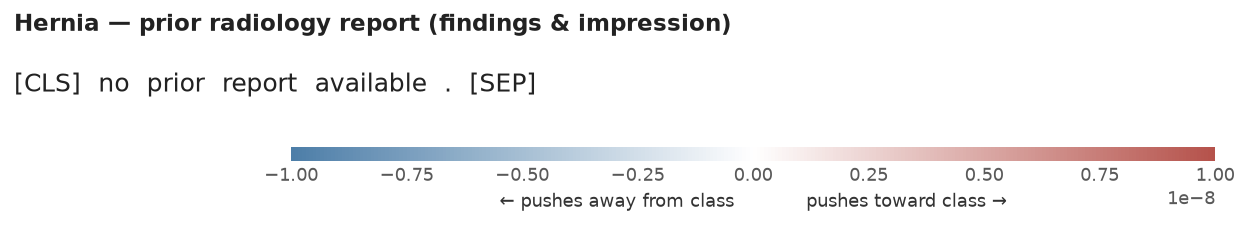
\includegraphics[width=0.85\textwidth]{img/hernia_text.png}
    \caption[Word-Level Clinical Text Attributions for Hernia]{Word-Level Clinical Text Attributions for Hernia.}
    \label{fig:hernia_text}
\end{figure}

\begin{figure}[H]
    \centering
    \begin{subfigure}[b]{0.48\textwidth}
        \centering
        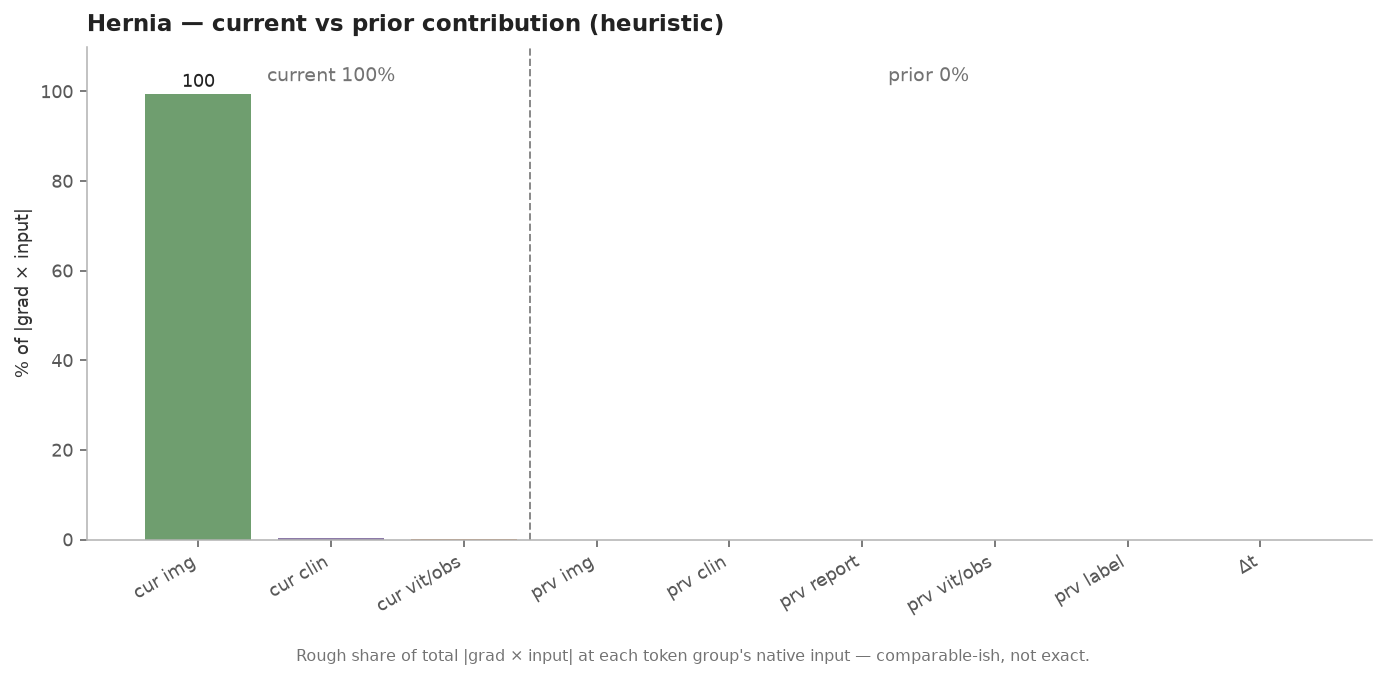
\includegraphics[width=\textwidth]{img/hernia_modality.png}
        \caption{Normal Scale}
        \label{fig:hernia_modality_normal}
    \end{subfigure}
    \hfill
    \begin{subfigure}[b]{0.48\textwidth}
        \centering
        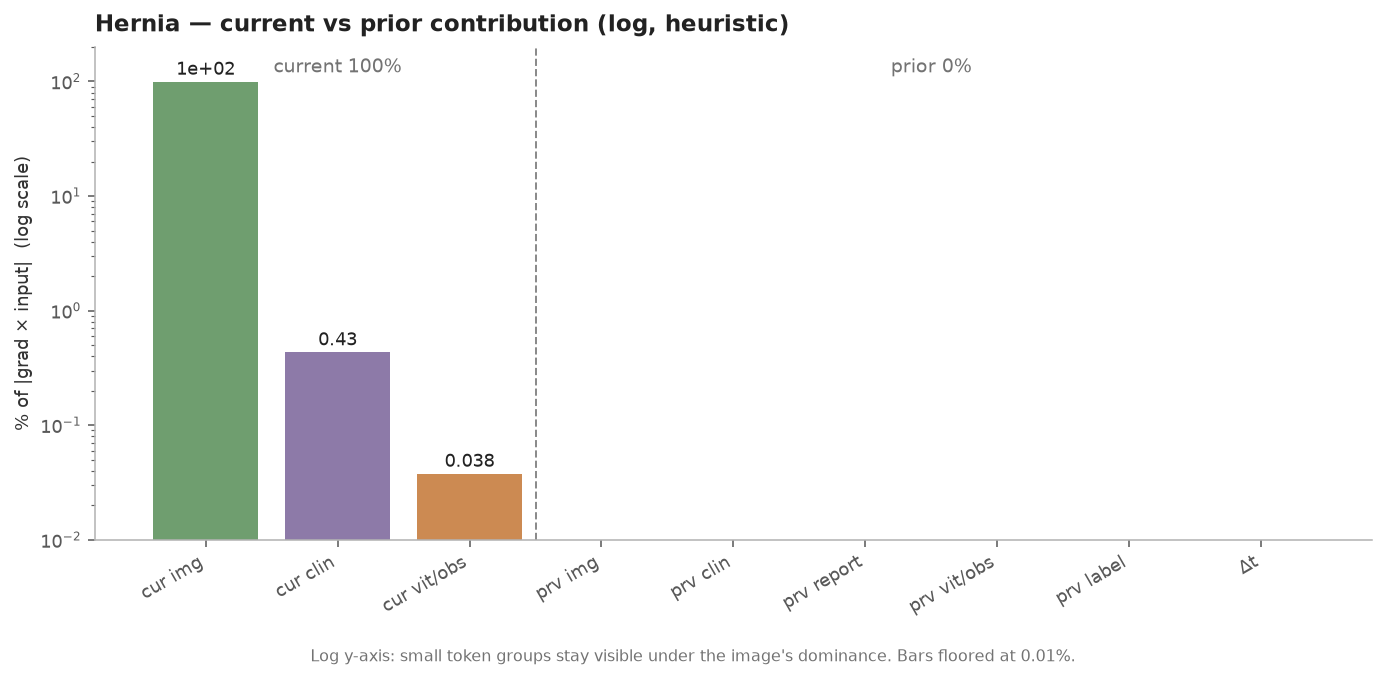
\includegraphics[width=\textwidth]{img/hernia_modality_log.png}
        \caption{Log Scale}
        \label{fig:hernia_modality_log}
    \end{subfigure}
    \caption[Modality Attribution Share for Hernia]{Modality Attribution Share for Hernia. (a) Normal scale. (b) Log scale.}
    \label{fig:hernia_modality}
\end{figure}
